\documentclass[border=8pt,varwidth=16cm]{standalone}
\usepackage[utf8]{inputenc}
\usepackage[T1]{fontenc}
\usepackage[turkish,shorthands=:!]{babel}
\usepackage{lmodern}
\usepackage{amsmath}
\usepackage{tikz}
\usetikzlibrary{arrows.meta,positioning,babel}
\usepackage[american]{circuitikz}
\begin{document}
\begin{minipage}{16cm}
\begin{minipage}{0.42\linewidth}
\centering
\begin{circuitikz}[thick]
  \draw (0,0) to[V, l=$V$, invert] (0,3)
        to[R, l=$R$, i>^=$i$] (2.6,3)
        to[L, l=$L$] (4.2,3) -- (4.2,2.15);
  \draw (4.2,1.5) circle (0.65) node {M};
  \draw (4.2,0.85) -- (4.2,0) -- (0,0);
  \node[font=\footnotesize, align=left] at (3.1,1.5) {$+$\\[-1pt]$K\dot\theta$\\[-1pt]$-$};
\end{circuitikz}

\small (a) elektrik kısmı
\end{minipage}%
\hfill
\begin{minipage}{0.52\linewidth}
\centering
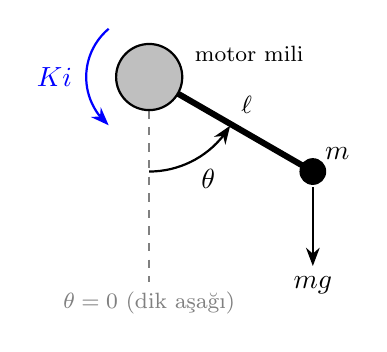
\begin{tikzpicture}[thick, >=Stealth]
  \draw[dashed, gray] (0,0) -- (0,-2.6) node[below, font=\footnotesize]{$\theta = 0$ (dik aşağı)};
  \draw[line width=2.2pt] (0,0) -- ({2.4*sin(60)},{-2.4*cos(60)})
        node[midway, above right=-1pt, font=\small]{$\ell$};
  \fill[gray!50, draw=black] (0,0) circle (0.42);
  \node[font=\footnotesize, right] at (0.45,0.3) {motor mili};
  \fill ({2.4*sin(60)},{-2.4*cos(60)}) circle (0.17)
        node[above right=1pt]{$m$};
  \draw[->] ({2.4*sin(60)},{-2.4*cos(60)-0.2}) -- ++(0,-1.0) node[below]{$mg$};
  \draw[->] (0,-1.2) arc[start angle=-90, end angle=-31, radius=1.2];
  \node at (-60:1.5) {$\theta$};
  \draw[->, blue] (130:0.8) arc[start angle=130, end angle=230, radius=0.8];
  \node[blue, left] at (180:0.85) {$K i$};
\end{tikzpicture}

\small (b) mekanik kısım (motor mili + kol)
\end{minipage}
\end{minipage}
\end{document}
